\chapter{Recursie}
Als we als programmeur een stuk code verschillende keren willen herhalen, hebben we tot nu toe telkens een lus gebruikt. We hebben een for-lus om een stuk code een bepaald aantal keer uit te voeren, en een while-lus om een stuk code uit te voeren totdat een bepaald stopcriterium bereikt wordt. Zo kunnen we bijvoorbeeld het probleem ``schrijf een stuk code dat alle getallen van 0 tot en met n optelt (voor n >= 0)'' heel gemakkelijk oplossen met een for-lus:

\examplecode{Recursie/telop.js}

Als we echter het probleem van naderbij bekijken, merken we op dat de eerste waarden van n, de volgende uitkomsten hebben:

\begin{itemize}
\item[] telOp(0) = 0
\item[] telOp(1) = 0+1
\item[] telOp(2) = 0+1+2 = 3
\item[] telOp(3) = 0+1+2+3 = 6
\item[] telOp(4) = 0+1+2+3+4 = 10
\item[] telOp(5) = 0+1+2+3+4+5 = 15
\item[] ...
\end{itemize}

Door deze uitwerkingen ondereen te zetten, zien we dat er een zekere overlap is tussen de verschillende berekeningen. Zo zien we bijvoorbeeld dat de berekening van telOp(3) volledig terugkomt in telOp(4), en dat de berekening van telOp(4) ook volledig terugkomt in telOp(5). We kunnen dus eigenlijk de vorige berekeningen ook omschrijven als volgt:

\begin{itemize}
\item[] telOp(0) = 0
\item[] telOp(1) = telOp(0)+1 = 1
\item[] telOp(2) = telOp(1)+2 = 3
\item[] telOp(3) = telOp(2)+3 = 6
\item[] telOp(4) = telOp(3)+4 = 10
\item[] telOp(5) = telOp(4)+5 = 15
\item[] ...
\end{itemize}

In het algemeen kunnen we zeggen dat telOp(n) berekend kan worden als volgt: telOp(n) = telOp(n-1)+n. Deze regel werkt voor elke waarde van n, behalve voor de waarde n=0 (aangezien telOp(-1) niet gedefinieerd is). Merk op dat de algemene regel om telOp te berekenen zelf gebruik maakt van telOp (weliswaar met een andere waarde). Dit is de essentie van recursie: ``een constructie die optreedt als onderdeel van zichzelf''. Deze regel levert ons de recursieve definitie op van het probleem:

\begin{quote}
\textbf{Voor alle n >= 0:} \\
n = 0:  telOp(n) = 0 \\
n > 0:  telOp(n) = telOp(n-1) + n
\end{quote}

We zien dat het probleem dus in twee delen opgedeeld wordt: de algemene regel waarmee we het resultaat kunnen berekenen voor bijna elke mogelijke waarde van n, en het basisgeval dat de oplossing geeft voor dat ene geval waar de algemene regel niet werkt.

\section{Recursieve functies}
We kunnen recursie ook gebruiken tijdens het programmeren. Een functie die zichzelf (rechtstreeks of onrechtstreeks) oproept, noemen we een recursieve functie. We kunnen de functie van in de vorige sectie recursief schrijven als volgt:

\examplecode{Recursie/teloprec.js}

De implementatie van deze functie volgt quasi direct uit de recursieve definitie die we eerder opgesteld hebben. Indien n = 0, dan zitten we in het basisgeval (waar we dus de algemene regel niet kunnen gebruiken). In dit geval geven we onmiddellijk het resultaat terug aan de oproeper van de functie. In het andere geval moeten we het resultaat berekenen volgens de algemene regel. Het resultaat wordt dus berekend door telOp opnieuw op te roepen, maar deze keer met als argument n-1 in plaats van n. Deze functieoproep zal een resultaat teruggeven (de waarde van telOp(n-1)), en hierbij moeten we n bijtellen om de correcte waarde van telOp(n) te berekenen.

We gaan nu als voorbeeld eens kijken hoe de computer het resultaat berekent van telOp(2). Figuur~\ref{fig:vbrecursief} geeft schematisch weer hoe het algoritme uitgevoerd zal worden, en duidt ook expliciet vier stappen aan die belangrijk zijn in ons recursieve verhaal. De functie wordt door de gebruiker opgeroepen waarbij de parameter n de waarde 2 heeft. De computer zal de code uit de functie telOp beginnen uit te voeren, en zal dus eerst een functievariabele aanmaken en dan de waarde vergelijken met 0. Aangezien n = 2 zal dus niet voldaan zijn aan de conditie van de if en zullen wel dus in het else-gedeelte terecht komen. De functie gaat nu het gevraagde resultaat berekenen door eerste het resultaat van telOp(1) te berekenen, en daar dan n bij op te tellen. Wanneer de computer echter komt bij de lijn waar telOp(1) berekend wordt (stap A in het schema), dan gebeurt het volgende: de uitvoering van de eerste oproep van de telOp-methode wordt gepauzeerd, en de telOp-functie wordt opnieuw opgeroepen van begin af aan (maar deze keer met de waarde van n die op 1 staat, in plaats van op 2). Het is belangrijk om in te zien dat dit in feite overeenkomt met een kopie van de functie. Dit wil zeggen dat de code van de functie nog altijd hetzelfde is, maar de variabele resultaat in de tweede oproep van de telOp-functie is niet dezelfde variabele als de variabele resultaat van de eerste oproep! De tweede oproep werkt dus eigenlijk helemaal onafhankelijk van de eerste oproep.

\begin{figure}
\centering
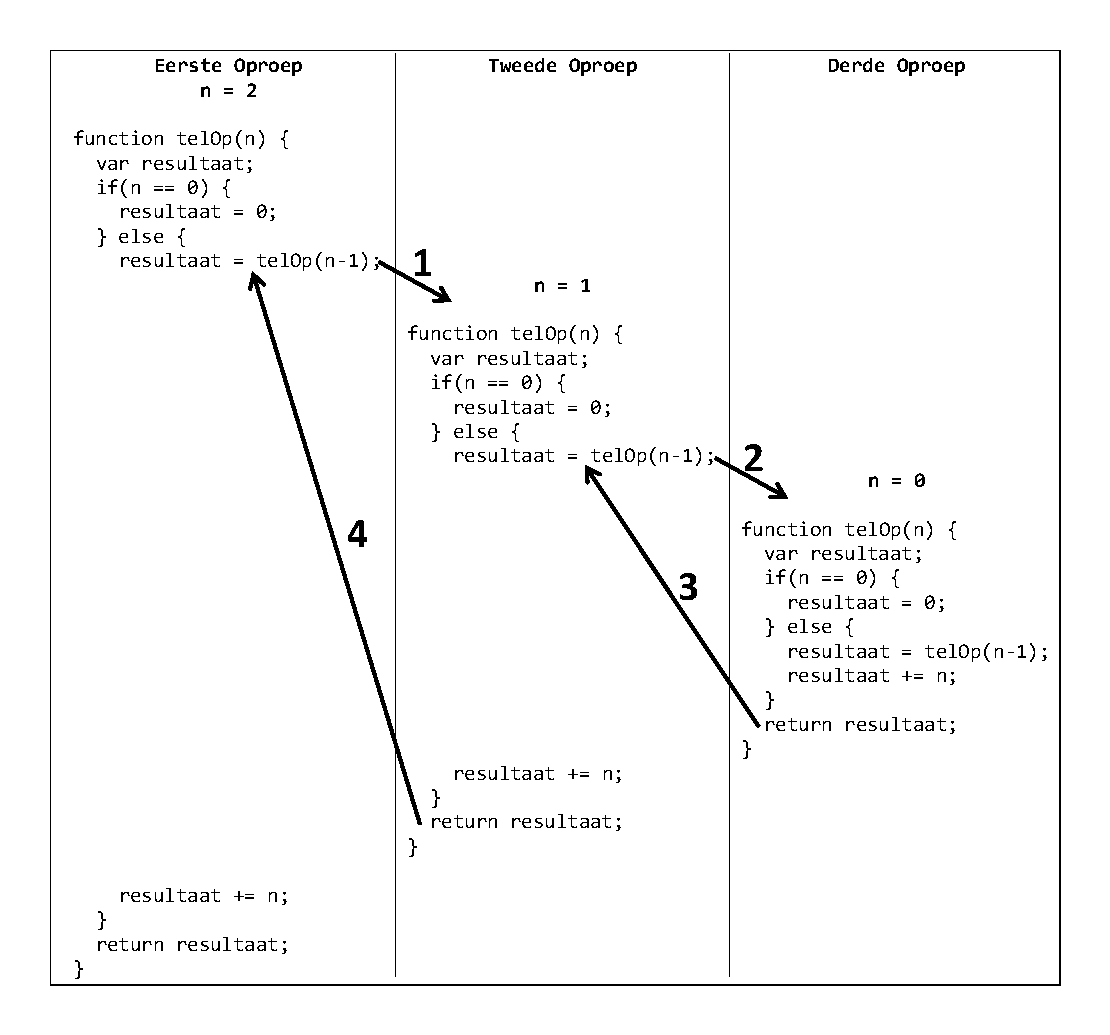
\includegraphics[scale=0.8]{Recursie/vb.pdf}
\caption{Een recursieve oproep.}\label{fig:vbrecursief}
\end{figure}

De tweede oproep begint dan uit te voeren om telOp(1) te berekenen. Ook hier wordt 1 vergeleken met 0, en komt de computer in de else terecht. Om het resultaat van telOp(1) te berekenen, zal de computer dus eerst telOp(0) berekenen (stap B in de tabel) en daarna hier 1 bij optellen. Net zoals eerder zal de berekening van telOp(0) er voor zorgen dat de tweede oproep tijdelijk gepauzeerd wordt, zodat de derde oproep zijn resultaat kan berekenen.

Bij de derde oproep is n = 0 geworden, en komen we dus terecht in ons basisgeval. Dit wil zeggen dat n vergeleken gaat worden met 0, en dat deze keer de conditie van de if zal gelden. De processor zal aan de variabele resultaat de waarde 0 toekennen (let op: de variabele resultaat van de derde oproep is niet dezelfde variabele als resultaat in de tweede of eerste oproep!), en dan later in stap C deze waarde teruggeven naar de tweede oproep.

Na stap C wordt de teruggeefwaarde van de derde oproep (de waarde 0) opgeslaan in de variabele resultaat van de tweede oproep. Nu kan de tweede oproep terug verder beginnen uit te voeren en zal dus de waarde van n (in de tweede oproep is n = 1) optellen bij resultaat. De uiteindelijke waarde van resultaat is dus 1, en wordt teruggegeven als teruggeefwaarde in stap D.

Nu kan de eerste oproep ook terug verder gaan met zijn berekening. De teruggeefwaarde van de tweede oproep (de waarde 1) wordt na stap D opgeslagen in de variabele resultaat, en bij deze variabele wordt da in de volgende lijn de waarde van n bij opgeteld. Aangezien in de eerste oproep de waarde van n = 2, is de eindwaarde van resultaat dus 3. Deze waarde wordt dan ook teruggegeven aan de gebruiker.

\section{Algemene kenmerken}

Recursie en lussen zijn sterk verbonden met elkaar. Beide zijn manieren om een stuk code meermaals uit te voeren totdat een bepaald stopcriterium bereikt is. Bij lussen is dit stopcriterium expliciet aanwezig (bij de while, bijvoorbeeld, is het stopcriterium de voorwaarde van de while; van zodra deze voorwaarde evalueert naar false zal de lus stoppen). Bij recursie is het stopcriterium impliciet aanwezig, in de vorm van het basisgeval. Als de computer bij een recursieve berekening uiteindelijk terecht komt in het basisgeval, zal er geen nieuwe recursieve oproep meer gebeuren (aangezien het resultaat van het basisgeval gekend is) en stopt dus het herhaaldelijk uitvoeren van hetzelfde stuk code. Een recursieve functie waar het stopcriterium ontbreekt, zal nooit stoppen (en is dus eigenlijk hetzelfde als een oneindige lus).

Theoretisch gezien zijn lussen en recursieve oproepen equivalent. Dit wil zeggen dat een lus herschreven kan worden als een recursieve functie, en ook omgekeerd dat een recursieve functie kan herschreven worden als een lus. Het maakt dus in zekere zin niet uit of je iteratief werkt (d.w.z. met lussen) of recursief. Sommige problemen lenen zich eerder tot een iteratieve oplossingen, voor andere problemen is een recursieve oplossing eleganter.

Om iteratieve code om te zetten naar recursieve code, ga je best als volgt te werk. Probeer eerst de algemene regel van het probleem te ontdekken. Dit kan je doen door de oplossing te berekenen voor een aantal verschillende parameterwaardes van de functie en door te kijken hoe de functie werkt. Let vooral op de uitkomsten van opeenvolgende parameterwaardes (bijv. in vorig voorbeeld, kijk wat de uitkomst is voor n=2, 3 en 4) en zoek uit op welke manier deze waardes aan elkaar gelinkt zijn. Als je hier een bepaalde structuur in ziet, dan ben je al goed op weg om de algemene regel te vinden. Eenmaal je de algemene regel hebt, moet je nog uitzoeken voor welke invoerwaardes de regel niet geldt. Dit is dan het basisgeval (of eventueel verschillende basisgevallen).

Recursie heeft een aantal nadelen, waardoor het in de praktijk veel minder gebruikt wordt dan lussen. Recursieve code gebruikt veel meer geheugen en is trager dan iteratieve code. Dit komt omdat een recursieve oproep overeenkomt met telkens een nieuwe functie-oproep te doen. Elke functie-oproep heeft plaats in het geheugen nodig, en heeft wat tijd nodig om alles klaar te maken voor de uitvoering van de functie. Vandaar dat recursieve code altijd minder performant is dan iteratieve code. Daarnaast lijdt de leesbaarheid van de code ook vaak onder het gebruik van recursieve code. Sommige problemen hebben een mooie recursieve oplossing, maar meestal is de iteratieve oplossing veel duidelijker leesbaar. Voor de oplossingen van de oefeningen mag je telkens zelf kiezen of je recursieve of iteratieve code schrijft (tenzij het expliciet anders aangegeven staat, natuurlijk).

\section{Voorbeelden}

Hieronder volgen een aantal typische voorbeelden van problemen die gemakkelijk recursief opgelost kunnen worden.

\subsection{Faculteit}

De wiskundige bewerking `faculteit' (ook wel genoteerd door het symbool `!') heeft een belangrijke rol bij kansrekenen en statistiek. De operatie wordt als volgt gedefinieerd:

\begin{quote}
\textbf{Voor alle natuurlijke getallen n:} \\
n = 0:  fac(n) = 1 \\
n > 0:  fac(n) = n . (n-1) . \ldots . 1
\end{quote}

We zien dus dat deze operatie zeer gelijkaardig is aan de telOp-operatie die we eerder in dit hoofdstuk hebben uitgewerkt. In plaats van op te tellen moeten we nu echter vermenigvuldigen. De wiskundige definitie zegt dat 0! = 1. Met andere woorden, het basisgeval waarbij n = 0, moet als resultaat 1 teruggeven. Alle andere gevallen kunnen volgens de algemene regel worden berekend. Dit geeft de volgend resultaten:

\begin{itemize}
\item[] fac(0) = 1
\item[] fac(1) = 1.1 = 1        = 0! . 1
\item[] fac(2) = 1.1.2 = 2        = 1! . 2
\item[] fac(3) = 1.1.2.3 = 6        = 2! . 3
\item[] fac(4) = 1.1.2.3.4 = 24    = 3! . 4
\end{itemize}

Algemeen geeft dit de volgende recursieve definitie:

\begin{quote}
\textbf{Voor alle natuurlijke getallen n:} \\
n = 0:  fac(n) = 1 \\
n > 0:  fac(n) = n . fac(n - 1)
\end{quote}

\subsection{Grootste gemene deler (Euclides)}

Euclides was een Grieks geleerde die in de oudheid leefde en voor heel wat wiskundige contributies gezorgd heeft. Zo heeft hij bijvoorbeeld een algoritme uitgedacht om op een heel eenvoudige manier de grootste gemene deler van twee getallen te berekenen.

Stel dat je twee getallen hebt, a en b, en je wil berekenen wat de grootste gemene deler is van die twee getallen. Indien de getallen gelijk zijn (met andere woorden, a = b), dan kunnen we de grootste gemene deler gewoon geven zonder een berekening te doen. Logischerwijze is het resultaat dan gelijk aan het getal zelf. In het andere geval zal ofwel a strikt groter zijn dan b, of b strikt groter dan a, en zullen we de grootste gemene deler wel moeten gaan berekenen.

Euclides merkte twee dingen op die uiteindelijk zullen leiden naar een algoritme om de grootste gemene deler te berekenen. Ten eerste zag hij dat de grootste gemene deler van de twee getallen a en b (waarbij we er nu van uit gaan dat a strikt groter is dan b) gelijk is aan de grootste gemene deler van de twee getallen (a-b) en b. Met andere woorden, ggd(a, b) = ggd(a-b, b). Ten tweede merkte hij ook op dat indien we deze stap blijven herhalen, dat we dan uiteindelijk op een punt komen waar a = b wordt. Door deze twee observaties samen te leggen, zien we dat we na herhaaldelijke toepassing van de eerste stap uitkomen in een situatie waar a = b, en dat dit getal de grootste gemene deler dan moet zijn van te twee originele getallen a en b waar we bij begonnen zijn.

Bijvoorbeeld, als we de grootste gemene deler van de getallen 12 en 90 willen zoeken, dan moeten we de volgende stappen uitvoeren:

\begin{quote}
ggd(12, 90) = ggd(12, 78) = ggd(12, 66) = ggd(12, 54) = ggd(12, 42) = ggd(12, 30) = ggd(12, 18) = ggd(12, 6) = ggd(6, 6) = 6
\end{quote}

We kunnen dit algoritme recursief beschrijven als volgt:

\begin{quote}
\textbf{Voor alle natuurlijke getallen a en b:} \\
a = b:  ggd(a, b) = a \\
a > b:  ggd(a, b) = ggd(a-b, b) \\
a < b:  ggd(a, b) = ggd(a, b-a)
\end{quote}

Als a = b, dan zitten we in het basisgeval. De grootste gemene deler is dan eenvoudigweg gelijk aan a. Indien a niet gelijk is aan b, dan zitten we in \'e\'en van de twee recursieve definities.

\subsection{Fibonacci}

Leonardo van Pisa (beter bekend als Fibonacci) was een Italiaans wiskundige die in de middeleeuwen een grote invloed had op de wetenschap. Zo voerde hij bijvoorbeeld de Arabische cijfers in (de cijfers die we vandaag nog altijd gebruiken), inclusief het getal 0, ter vervanging van de Romeinse cijfers.

Fibonacci was ook ge\"interesseerd in het fokken van konijnen, en introduceerde een cijferreeks die het verloop van zijn konijnenpopulatie weergaf. Deze reeks, beter bekend als de rij van Fibonacci, heeft ook nog interessante toepassingen buiten het kweken van konijnen.

De rij ziet er als volgt uit: 0, 1, 1, 2, 3, 5, 8, 13, 21, 34, 55, 89, ...

We merken op dat een Fibonacci-getal kan berekend worden door de twee voorgaande Fibonacci-getallen op te tellen. Dit geeft ons meteen de algemene regel die voor alle Fibonacci-getallen kan toegepast worden, behalve voor de eerste twee getallen. Deze getallen hebben namelijk geen twee voorgangers. We hebben hiermee genoeg informatie om de recursieve definitie van het probleem op te stellen:

\begin{quote}
\textbf{Voor alle natuurlijke getallen n:} \\
n = 0:  fib(n) = 0 \\
n = 1:  fib(n) = 1 \\
n > 1:  fib(n) = fib(n-1) + fib(n-2)
\end{quote}

Onze recursieve definitie bestaat deze keer uit twee basisgevallen in plaats van \'e\'en. Zowel fib(0) als fib(1) kunnen we niet uitrekenen met de algemene regel en voor deze twee waardes moeten we dus een uitzondering maken.

\subsection{De torens van Hanoi}

De torens van Hanoi is een wiskundige puzzel die in 1883 in het Westen gepopulariseerd werd door \'Edouard Lucas. Het spel bestaat uit drie palen en een aantal schijven van een verschillende grootte. In de beginsituatie liggen alle schijven op elkaar rond de eerste paal. De grootste schijf ligt onderaan, de tweede grootste schijf daar boven, enz. De bedoeling is nu dat alle schijven van de eerste paal naar een andere paal verzet worden, maar er moet ten alle tijde wel aan de volgende regels voldaan worden:

\begin{enumerate}
\item In elke stap mag er hoogstens \'e\'en schijf verzet worden
\item Een grotere schijf mag nooit op een kleinere schijf liggen
\end{enumerate}

De begin- en eindsituatie van het spel worden afgebeeld in Figuur~\ref{fig:hanoi1}.

\begin{figure}
\centering
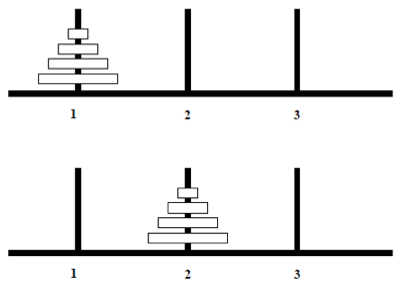
\includegraphics[scale=0.8]{Recursie/hanoi1.png}
\caption{Torens van Hanoi: begin- en eindsituatie}\label{fig:hanoi1}
\end{figure}

Een recursieve oplossingsstrategie is de volgende. Als we de vier schijven rond de eerste paal willen verplaatsen naar de tweede paal, dan moeten we dit probleem opsplitsen in gemakkelijkere deelproblemen. Wat we kunnen doen is eerste de drie bovenste schijven verzetten naar de derde paal (dit mag natuurlijk in \'e\'en stap!), dan verzetten we de vierde schijf naar de tweede paal, en daarna zetten we de drie schijven van de derde paal bovenop de schijf die al rond de tweede paal zat. Schematisch voeren we dus de operatie uit die afgebeeld staat in Figuur~\ref{fig:hanoi2}.

\begin{figure}
\centering
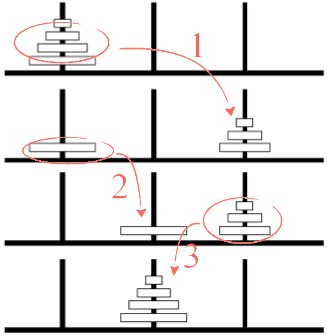
\includegraphics[scale=0.8]{Recursie/hanoi2a.png}
\caption{Torens van Hanoi: schematische weergave van het algoritme}\label{fig:hanoi2}
\end{figure}

We hebben ons probleem (``verzet vier schijven'') dus omgevormd tot een makkelijkere versie van het probleem (``verzet drie schijven, verzet \'e\'en schijf, verzet drie schijven''). Natuurlijk mogen die drie schijven niet in \'e\'en stap verzet worden, dus deze stap zullen we terug moeten opdelen in `makkelijkere' stappen. We kunnen hiervoor hetzelfde algoritme gebruiken, waarbij het probleem ``verzet drie schijven'' vereenvoudigd wordt tot ``verzet twee schijven, verzet de derde schijf, verzet twee schijven''. Dit is dus een recursieve oproep. Als we dit algoritme in JavaScript-code schrijven, krijgen we de volgende oplossing:

\examplecode{Recursie/hanoi.js}

De functie hanoi heeft drie parameters: hoogte die aangeeft hoeveel schijven er moeten verzet worden, van die de waarde bevat van de paal waar de schijven moeten gehaald worden (dit kan de waarde 1, 2 of 3 zijn), en naar die de waarde bevat van de paal waar de schijven naar verplaatst moeten worden. Indien er maar \'e\'en schijf verzet moet worden (als hoogte dus gelijk is aan 1), dan wordt die onmiddellijk verplaatst. De regels laten namelijk toe dat deze schijf direct verplaatst wordt. Als er meerdere schijven verplaatst moet worden (hoogte > 1), dan moeten we dit probleem opsplitsen in eenvoudigere problemen. In een eerste stap verzetten we (hoogte-1) schijven naar de reservepaal. Welke paal dit is kan eenvoudig berekend worden met de formule ``6 - van - naar''. Het verzetten van deze schijven doen we door een recursieve oproep (Stap 1 in het schema). Als deze recursieve oproep voltooid is, dan zijn er dus (hoogte-1) schijven verzet, en moeten we nog de laatste schijf verzetten. Dit kan direct gebeuren omdat de regels toelaten om \'e\'en schijf te verzetten (Stap 2 in het schema). Na deze stap moeten we de (hoogte-1) schijven zetten op de schijf die we net verzet hebben (Stap 3 in het schema). Ook dit doen we met een recursieve oproep.

%%% Local Variables: 
%%% mode: latex
%%% TeX-master: "../main"
%%% End: 
